%!TEX root = ../main-anran-ma.tex 
% so I can build in this tex file too. 
%************************************************
% \setcounter{theorem}{6}
\chapter{A Proof System}\label{ch:system} % $\mathbb{ZNR}$
%************************************************

\section{Literature Review}

Here is a description of all the triples. 
\todo{Literature review section}



We are interested in studying the \define{necessary liberal precondition}, a weakening of the weakest liberal precondition: 
$$wlp.C.F\implies G$$
The weaker $G$ can contain various preconditions: on the one hand, $G$ can be so general that it is satisfied by any program state; on the other hand, a $G$ that is barely weaker than $wlp.C.F$ is also not much different from the latter. 
Alternatively, $G$ can also contain all kinds of preconditions that starting from it, any postcondition is reachable. 
One thing we are certain about, though, is that a program with an original state satisfying $\neg G$ will terminate, and the final state can satisfy $\neg F$: 
\begin{align*}
wlp.C.F\implies G & = \neg G \implies \neg wlp.C.F \\
	& = \neg G \implies wp.C.\neg F 
	\hspace{0.3\textwidth} | \ \todo{insert theorem: wlp and wp are conjugates} 
\end{align*}
In the upcoming sections, we first discuss various forms that the necessary liberal precondition can take and try to identify a $G$ that is most characteristic. 
We proceed then to propose a proof system stemming from the necessary liberal precondition and show its usefulness using an example. \todo{replace with concrete example} 

\section{A Precondition Weaker Than the Weakest Liberal Precondition}
In \autoref{sec:wlp} we defined the weakest liberal precondition and state that it characterizes all the preconditions under whose control the program either \imptt{diverges} or \imptt{will} terminate in a state satisfying $F$. 
We are certain to use ``will'' instead of ``can'', because we view the non-determinism as demonic, so the behavior of wlp can be depicted by \autoref{subfig:wlpd}. 
We can categorize the executions of the program in four ways: 
\begin{enumerate}
	\item the dashed arrow means non-terminating executions; 
	\item the black arrows are executions starting from an initial state satisfying $wlp.C.F$ and only terminating in final states satisfying $F$; 
	\item the green arrows are the executions starting from an initial state satisfying $\neg wlp.C.F$ but can terminate in states either satisfying $F$ or satisfying $\neg F$;
	\item the red arrow represents executions starting from an initial state satisfying $\neg wlp.C.F$ and only terminating in final states satisfying $\neg F$. 
\end{enumerate}


\begin{figure}[ht!]\centering
	\subfloat[Weakest liberal precondition (demonic non-determinism)\label{subfig:wlpd}]{
		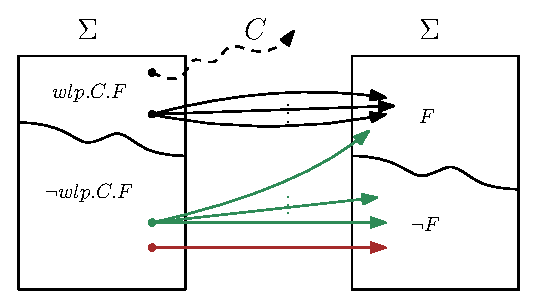
\includegraphics[width=0.4\textwidth]{image/wlp-g/wlpd.eps}}
	\hfill

	\subfloat[Precondition $G$ with $wlp.C.F\implies G$ and $G$ contains some green arrows\label{subfig:wlp-g-g}]{
		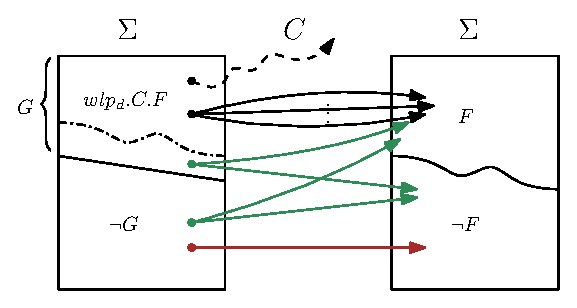
\includegraphics[width=0.45\textwidth]{image/wlp-g/wlp-g-g.eps}
	}
	\hfill
	\subfloat[Precondition $G$ with $wlp.C.F\implies G$ and $G$ contains all the green arrows\label{subfig:wlp-g-gg}]{
		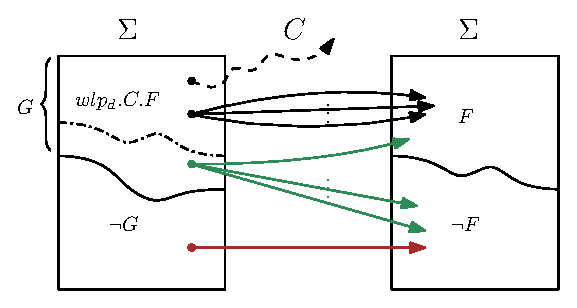
\includegraphics[width=0.45\textwidth]{image/wlp-g/wlp-g-gg.eps}
	}

	\subfloat[Precondition $G$ with $wlp.C.F\implies G$ and $G$ contains some red arrows\label{subfig:wlp-g-r}]{
		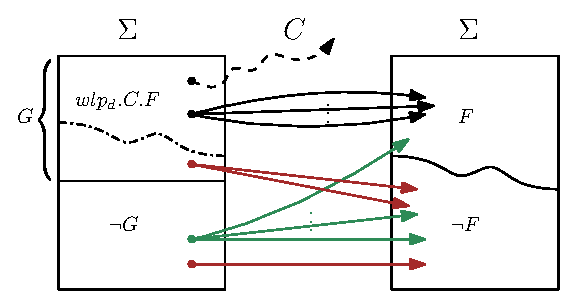
\includegraphics[width=0.45\textwidth]{image/wlp-g/wlp-g-r.eps}
	}
	\hfill
	\subfloat[Precondition $G$ with $wlp.C.F\implies G$ and $G$ contains all the red arrows\label{subfig:wlp-g-rr}]{
		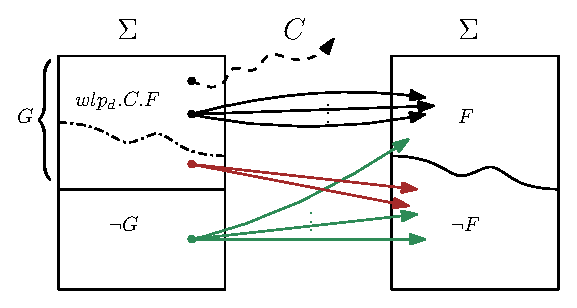
\includegraphics[width=0.45\textwidth]{image/wlp-g/wlp-g-rr.eps}
	}
\caption{Case Distinction of Preconditions Weaker Than wlp}
\label{fig:wlp-g-1}
\end{figure}

\begin{figure}[ht!]\centering
	\ContinuedFloat
	\subfloat[Precondition $G$ with $wlp.C.F\implies G$ and $G$ contains some green arrows and some red arrows\label{subfig:wlp-g-gr}]{
		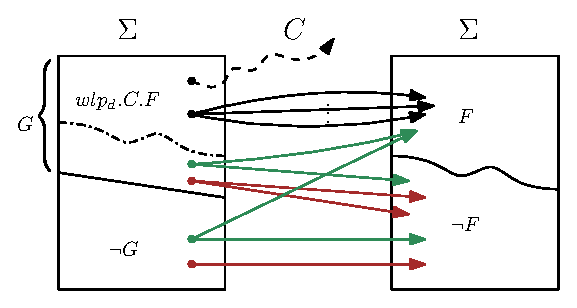
\includegraphics[width=0.45\textwidth]{image/wlp-g/wlp-g-gr.eps}
	}
	\hfill
	\subfloat[Precondition $G$ with $wlp.C.F\implies G$ and $G$ contains all the green arrows and some red arrows\label{subfig:wlp-g-ggr}]{
		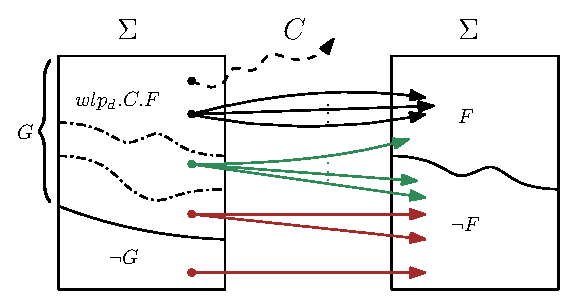
\includegraphics[width=0.45\textwidth]{image/wlp-g/wlp-g-ggr.eps}
	}

	\subfloat[Precondition $G$ with $wlp.C.F\implies G$ and $G$ contains some green arrows and all the red arrows\label{subfig:wlp-g-grr}]{
		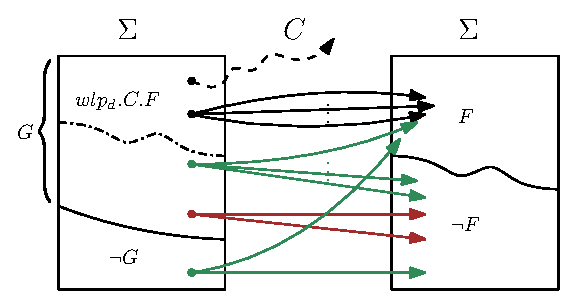
\includegraphics[width=0.45\textwidth]{image/wlp-g/wlp-g-grr.eps}
	}
	\hfill
	\subfloat[Precondition $G$ with $wlp.C.F\implies G$ and $G$ contains all the arrows\label{subfig:wlp-g-ggrr}]{
		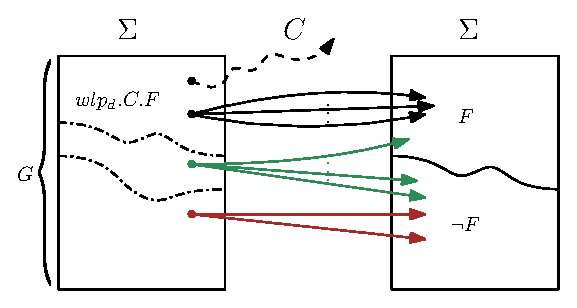
\includegraphics[width=0.45\textwidth]{image/wlp-g/wlp-g-ggrr.eps}
	}
\caption{Case Distinction of Preconditions Weaker Than wlp (Cont.) }
\label{fig:wlp-g-2}
\end{figure}
If we were to weaken the precondition, it can happen in various ways as shown in \autoref{subfig:wlp-g-g}{\color{RoyalBlue}-9}. 
However, $G$ spikes our interest when it takes the form as in \autoref{subfig:wlp-g-gg}, because under its control, the program always \imptt{can} reach a final state satisfying $F$ if it terminates, while with an initial state satisfying $\neg G$, the program is \imptt{will} terminate satisfying $\neg F$. 
This behavior is exactly the behavior of wlp, if we were to regard the non-deterministic choice as angelic, as hinted by the similarities between \autoref{subfig:wlp-g-gg} and \autoref{subfig:wp-angelic}. 
We thus first investigate this special case, before proceeding with $G$ in general. 

\subsection{A Special Case} %: $G$ is wlp with Angelic Non-determinism
Dual to the semantics of wp and wlp as shown in \thm{wp-sound} and \thm{wlp-sound}, we can deduce the semantics of wlp with angelic non-determinism (denoted by \define{wlp$_a$}) recalling the representation for non-termination mentioned in \autoref{sec:big-step}: 
\begin{statement}{wlpa-sound}[Semantics of $wlp_a$]
\ \vspace{-1.5mm}
\[
wlp_a.C.F = \{ \sigma\in\S \mid
\neg(\exists \tau\in\S: \sigma\goto{C}\tau) \ \ \vee\ \ 
(\exists \tau\in\S: \sigma\goto{C}\tau\wedge  \tau\vDash F)
 \}
\]
% \label{thm:wlpa}
\end{statement}

Luckily, we can find statements using wlp and sp that captures this specific $G$, hence giving us a way to express wlp$_a$ without having to define it: 
\begin{lemma}{wlpa-g}[Angelic wlp implies G]
\ \\ \vspace{-3mm}
	\[\hspace{-2mm}
	\text{ if \ \ \ \ } 
	(wlp.C.F\implies G)
	\ \wedge\ 
	(sp.C.\neg G \implies \neg F) 
	\text{\ \ \ \  then\ \ \ \  } 
	wlp_a.C.F \implies G
	\] 
	\label{lem:wlp-g}
\end{lemma}
The second prerequisite \mathl{sp.C.\neg G \implies \neg F } states that from $\neg G$ we are only allowed to reach $\neg F$, making sure that all green arrows as in \autoref{fig:wlp-g-1} are included in $G$. 

% macros for referencing to lines in this chapter
\newcommand{\lblth}[1]{\hypertarget{3.#1}{{\text{#1}}}}
\newcommand{\refth}[1]{\hyperlink{3.#1}{{\text{Line (#1)}}}}
\begin{proof}
	The assumption expresses that for any state $\sigma\in\S$:
\begin{align*} 
	wlp.C.F\implies G\  \Leftrightarrow&\ \sigma\in wlp.C.F \implies \sigma\in G \\
	\Leftrightarrow&\ ( \forall \tau\in\S:\ \sigma\goto{C}\tau\implies  \tau\in F) \implies \sigma\in G \tag*{$\mid$ \thm{wlp-sound}} \\
	\Leftrightarrow&\ (\forall \tau\in\S:\ \neg(\sigma\goto{C}\tau)\ \vee\ \tau\in F) \implies \sigma\in G \\
	\Leftrightarrow&\ \neg(\exists\tau\in\S:(\sigma\goto{C}\tau)\ \wedge\ \neg(\tau\in F)) \implies \sigma\in G \tag{\lblth{a}} \\
	% && \mid \lblth{a} \\
	% &\ \ \ \  \vee (\forall \tau.\sigma\goto{C}\tau:\tau\in F \Longrightarrow \sigma\in G) 
		% \hspace{0.017\textwidth} \mid \lblth{b} \\
	%
\end{align*}
Also, for any state $\tau\in\S$: 
\begin{align*}
	sp.C.\neg G \implies \neg F \Leftrightarrow&\ \tau\in sp.C.\neg G \implies \tau\in \neg F \\
	\Leftrightarrow&\  (\exists \mu\in\S:\ \mu\goto{C}\tau\ \wedge\ \mu\in\neg G )\implies \tau\in\neg F \tag*{$\mid$ \thm{sp-sound}}\\
	% &\hspace{0.45\textwidth} \mid \thm{sp-sound}\\
	\Leftrightarrow&\  \neg (\tau\in\neg F) \implies \neg (\exists \mu\in\S:\ \mu\goto{C}\tau\ \wedge\ \mu\in\neg G ) \\
	\Leftrightarrow&\  \tau\in F \implies \forall \mu\in\S:\ \neg (\mu\goto{C}\tau\ \wedge\ \mu\in\neg G)\\
	\Leftrightarrow&\  \tau\in F \implies \forall \mu\in\S:\ \neg (\mu\goto{C}\tau)\ \vee\ \neg(\mu\in\neg G)\\
	\Leftrightarrow&\  \tau\in F \implies \forall \mu\in\S:\ \neg (\mu\goto{C}\tau)\ \vee\ \mu\in G
	\tag{\lblth{b}} \\
	%
\end{align*}
Our goal is to prove that for any state $\sigma\in\S$:
\begin{align*}
	wlp_a.C.F \implies G \Leftrightarrow&\ \sigma\in wlp_a.C.F \implies \sigma\in G \\
	\Leftrightarrow&\  \neg(\exists \tau\in\S: \sigma\goto{C}\tau) \ \vee\ 
	(\exists \tau\in\S: \sigma\goto{C}\tau\wedge  \tau\in F)\\
	&\ \ \ \ \implies \sigma\in G \tag*{$\mid$ \stm{wlpa-sound}}\\
	% &\hspace{0.45\textwidth} \mid \stm{wlpa-sound}\\
	\Leftrightarrow&\  (\neg(\exists \tau\in\S: \sigma\goto{C}\tau)\implies \sigma\in G ) \tag{\lblth{c}}\\
	% && \mid \lblth{c}\\
	&\ \wedge\ ((\exists \tau\in\S: \sigma\goto{C}\tau\wedge  \tau\in F)\implies\sigma\in G) \tag{\lblth{d}}\\
	% && \mid \lblth{d}
\end{align*}
We can prove \lem{wlpa-g} by proving that \refth{a} implies \refth{c} and that \refth{b} implies \refth{d}.
For any state $\sigma\in\S$, we first prove (a)$\implies$(c):
\begin{align*}
	% \text{(a)}\implies\text{(c)}:\text{ for any } \\
	true 
	\Leftrightarrow&\ (\exists\tau\in\S:(\sigma\goto{C}\tau)\ \wedge\ \neg(\tau\in F)) \implies (\exists\tau\in\S:\sigma\goto{C}\tau)\\ 
	\Leftrightarrow&\ \neg(\exists\tau\in\S:\sigma\goto{C}\tau) \implies \neg(\exists\tau\in\S:(\sigma\goto{C}\tau)\ \wedge\ \neg(\tau\in F))  \\ 
	\Rightarrow&\ \neg(\exists\tau\in\S:\sigma\goto{C}\tau) \implies \sigma\in G \tag*{$\mid$ \refth{a}}\\
\end{align*}
It is also valid that for any state $\sigma\in\S$, (b)$\implies$(d). 
Assume there exists $\tau\in\S$ such that for some state $\sigma\in\S$, 
$$\sigma\goto{C}\tau\ \wedge\  \tau\in F \text{ is valid. }$$
Then we conclude from \refth{b} that 
$$\forall \mu\in\S:\ \neg (\mu\goto{C}\tau)\ \vee\ \mu\in G$$
Since $\sigma\in\S$, it follows that $\neg(\sigma\goto{C}\tau)\ \vee\ \sigma\in G$. 
We already know that $\sigma\goto{C}\tau$, hence $\sigma\in G$ must be true, therefore proving \refth{d}. 
\end{proof}


\begin{lemma}{g-wlpa}[G implies angelic wlp]
\ \\ \vspace{-3mm}
	\[%\hspace{-5mm}
	\text{ if \ \ \ \ } 
	(P{\implies} G) \implies \neg(sp.C.P {\implies} \neg F)
	\text{\ \ \ \  then\ \ \ \  } 
	G {\implies} wlp_a.C.F
	\] 
\end{lemma}
Here, the prerequisite states that we do not allow executions starting from $G$ that \imptt{only} finish in $\neg F$, making sure that $G$ does not include the red arrows as in \autoref{fig:wlp-g-1}.  

\begin{proof}
	The assumption expresses that for any state $\sigma\in\S$:
\begin{align*} 
	&\ P\implies G \implies \neg(sp.C.P \implies \neg F) \\ 
	\Leftrightarrow&\ P\implies G \implies \neg(\forall\tau\in\S:\tau\in sp.C.P{\implies}\tau\in\neg F) \\ 
	\Leftrightarrow&\ P\implies G \implies \exists\tau\in\S:\neg(\tau\in sp.C.P{\implies}\tau\in\neg F) \\ 
	\Leftrightarrow&\ P\implies G \implies \exists\tau\in\S:\tau\in sp.C.P\ \wedge\ \neg(\tau\in\neg F) \\ 
	\Leftrightarrow&\ P\implies G \implies \exists\tau\in\S:\tau\in sp.C.P\ \wedge\ \tau\in F \\ 
	\Leftrightarrow&\ P\implies G \implies \exists\tau\in\S:(\exists \mu\in\S:\ \mu\goto{C}\tau\ \wedge\ \mu\in P)\ \wedge\ \tau\in F \tag*{$\mid$ \thm{sp-sound}}\\ 
	\Leftrightarrow&\ \sigma\in P {\implies} \sigma\in G {\implies} \exists\tau\in\S:(\exists \mu\in\S:\ \mu\goto{C}\tau\ \wedge\ \mu\in P)\ \wedge\ \tau\in F \tag{\lblth{e}}\\ 
	%
\end{align*}
Our goal is to prove that for any state $\sigma\in\S$:
\begin{align*}
	&\ G\implies wlp_a.C.F \\ 
	\Leftrightarrow&\  \sigma\in G\implies\sigma\in wlp_a.C.F\\
	\Leftrightarrow&\ \sigma\in G\implies \neg(\exists \tau\in\S: \sigma\goto{C}\tau) \ \vee\ 
	(\exists \tau\in\S: \sigma\goto{C}\tau\wedge  \tau\in F) \tag*{$\mid$ \stm{wlpa-sound}}\\
\end{align*}
For some state $\sigma\in\S$, assume $\sigma\in G$, then we can construct set $P=\{\sigma\}$ such that the prerequisites in \refth{e} holds. 
Consequently, the postrequisite in holds. 
Now we can find witnesses $\mu$ and $\tau$ such that
$$
\mu\goto{C}\tau\ \wedge\ \mu\in P\ \wedge\ \tau\in F 
$$
Since $P$ is a singleton set, $\mu$ can only be $\sigma$. 
Then we have found a witness $\tau$ such that $\sigma\goto{C}\tau$ and $\tau\in F$, satisfying the postrequisite of our goal. 
\end{proof}

\begin{corollary}{g=wlp}[G equivalent to angelic wlp]
% \begin{align*}
	\ \\
	$\text{ if } \ wlp.C.F{\implies} G \ \wedge\ 
	sp.C.\neg G {\implies} \neg F 
	\ \text{ and } \ 
	P{\implies} G \implies \neg(sp.C.P {\implies} \neg F) \\
	\text{ then }\ G = wlp_a.C.F$
% \end{align*}	
\end{corollary}

\subsection{The General Case}
While having restrictions on $G$ yields interesting results, without the restrictions we can still find useful characteristics. 
As shown in \autoref{fig:wlp-g-2}, $G$ can contain all possible initial states, which can be the starting points of black, green, red, or dashed arrows, representing executions terminating in states satisfying $F$, $F$ or $\neg F$, $\neg F$, or non-terminating, respectively. 
As a result, we can not make much statements without adding extra restrictions to $G$. 
However, we can see from \autoref{fig:wlp-g-2} that $\neg G$ does not contain any \imptt{black} or \imptt{dashed} arrows in all cases. 
In other words, if program $C$ starts in any initial state satisfying $\neg G$, then 
\begin{itemize}
	\item its executions terminate, and
	\item there exists an execution that ends up in a final state that satisfies $\neg F$. 
\end{itemize}

This corresponds to the semantics of the wp transformer as shown in \thm{wp-sound}, hinting that \hoare{\neg G}{C}{\neg F} is a valid Hoare triple. 
The question then naturally arises: why do we concern ourselves with $G$, if we can just prove our specifications using wp or Hoare triples? 
To demonstrate the answer, we analyze the example written in \autoref{lst:pererson}. 

\todo{consider listing numbering to follow figures?}
\begin{lstlisting}[caption={Thread $A$ Hoping to Access Critical Section}, label={lst:pererson}, language=java, numbers=left, stepnumber=1, captionpos=b,escapechar=|,frame=single]
	... // leave non-critical section
	turn := B; |\label{line:p-2}|
	while (turn != A) do 
		turn := A |$\square$| turn := B |\label{line:p-4}|
		// modeling the behavior of other threads
	critA := true;|\label{line:p-6}|
	... // enter critical section  
\end{lstlisting}

The pseudocode is modified from Peterson's mutual exclusion algorithm~\cite{peterson1981}, but we are now only concerned with one of possibly many threads.
Our thread $A$ is trying to enter some critical section but only have limited knowledge as to what other threads might also want to access the same critical section: $A$ is only aware of thread $B$ that also wants to enter critical section. 

To have a \imptt{fair} system, thread $A$ gives $B$ the turn after leaving non-critical section as written in \moreref{line}{line:p-2} of \autoref{lst:pererson}. 
Otherwise, thread $A$ might never enter the while-loop and directly skip ahead to \moreref{line}{line:p-6} to enter the critical section, without giving other threads a chance. 
\moreref{Line}{line:p-4} models the behavior of other threads in the system: while $A$ is waiting for its turn, thread $B$ might also have just left the non-critical section and gave the turn to $A$; or some other thread than $A$ or $B$ might have given the turn to $B$.~\footnote{We will see with the calculation for wlp of this while-loop that it makes no difference whether we include more non-deterministic choices like $turn := C\ \square\ turn := D\ \square\ \dots$.} 

Mutual exclusion requires that no threads are simultaneously in the critical section. 
In this case, a state we definitely want to avoid is where the values of $critA$ and $critB$ are both true. 
In other words, the postcondition 
$$F=\{\sigma\in\S\mid \sigma.critB=true\}$$ 
after \moreref{line}{line:p-6} in \autoref{lst:pererson} is an undesirable postcondition.

Filling in this $F$ after \moreref{line}{line:p-6} and calculating the weakest liberal precondition backwards according to \autoref{tab:wp-wlp}, we arrive at the conditions as shown in \autoref{lst:critB}. 
For better readability, we shorten predicates like $F$ to $\{critB\}$.

\begin{lstlisting}[caption={Weakest Liberal Precondition w.r.t Postcondition $F=\{\sigma\in\S\mid \sigma.critB=true\}$ }, label={lst:critB}, language=java, numbers=left, stepnumber=1, captionpos=b,escapechar=|,frame=single]
	... // leave non-critical section
	|\imptt{\{critB\}}|
	turn := B;
	|\imptt{\{critB\}}\label{line:c-4}|
	while (turn != A) do 
		turn := A |$\square$| turn := B 
		// modeling the behavior of other threads
	|\imptt{\{critB\}}\label{line:c-8}|
	critA := true;
	|\imptt{\{critB\}}|
	... // enter critical section  
\end{lstlisting}

The only non-obvious step in \autoref{lst:critB} is from \moreref{line}{line:c-8} to \moreref{line}{line:c-4}. 
Remember from \autoref{tab:wp-wlp} that the wlp for while-loops is defined with the greatest fixed point operator: 
\[
	wlp.(\text{while }(\varphi)\ \{C'\}).F = gfp\ X.\ (\neg\varphi\wedge F)\vee(\varphi\wedge wlp.C'.X)
\]
We simply follow the iteration to find the greatest fixed point of a function until we see a pattern, then prove by natural induction that the solution we found is indeed the greatest fixed point. \todo{Define and refer to the iteration from top. }

\begin{lemma}{critB}
	$wlp.WHILE.\{critB\} = \{critB\}$
	where $WHILE := while\ (\varphi)\ do\ C'$, $\varphi := \{turn!=A\}$,\ \ and $C':=(turn:=A\ \square\ turn:=B)$. 
\end{lemma}
\begin{proof} 
	\begin{align*}
		\text{Let }\Phi(X) :=&\ \neg\varphi\wedge F\ \ \vee\ \ \varphi\wedge wlp.C'.X\\ 
		=&\ \{turn=A\}\wedge \{critB\}\ \ \vee\ \ \{turn!=A\} \wedge wlp.C'.X\\
		\text{Then }\Phi(true) =&\ \{turn=A\}\wedge \{critB\}\ \ \vee\ \ \{turn!=A\} \wedge wlp.C'.true \\ 
		\overset{\thm{wlp-true}}{=}&\ \{turn=A\}\wedge \{critB\}\ \ \vee\ \ \{turn!=A\} \wedge true \\
		% &\hspace{0.45\textwidth} | \ \thm{wlp-true} \\
		=&\ \{turn != A\} \vee \{critB\} \\
	\end{align*}
	\begin{align*}
		\text{Also, } wlp.C'.\Phi(True)=&\ wlp.(turn:=A\ \square\ turn:=B).\Phi(true)\\
		\overset{\autoref{tab:wp-wlp}}{=}&\ wlp.(turn:=A).(\{turn != A\} \vee \{critB\}) \\
		&\ \wedge wlp.(turn:=B).(\{turn != A\} \vee \{critB\})\\
		\overset{\autoref{tab:wp-wlp}}{=}&\ (\{A!=A\}\vee\{critB\})\wedge\{B!=A\}\vee\{critB\}\\
		=&\ \{critB\}\wedge true \\
		=&\ \{critB\}
	\end{align*}
	\begin{align*}
		\text{Hence, }\Phi^2(true) =&\ \{turn:=A\}\wedge \{critB\}\\
		&\ \vee\ \ \{turn!=A\} \wedge wlp.C'.\Phi(true) \\
		=&\ \{turn:=A\}\wedge \{critB\}\ \ \vee\ \ \{turn!=A\} \wedge \{critB\}\\
		=&\ \{critB\} \wedge (\{turn:=A\} \vee \{turn!=A\})\\
		=&\ \{critB\}\\
		\text{And } wlp.C'.\Phi^2(True)=&\ wlp.(turn:=A\ \square\ turn:=B).\Phi^2(true)\\
		\overset{\autoref{tab:wp-wlp}}{=}&\ wlp.(turn:=A).\{critB\} \\
		&\ \wedge wlp.(turn:=B).\{critB\}\\
		\overset{\autoref{tab:wp-wlp}}{=}&\ \{critB\}\wedge\{critB\}\\
		=&\ \{critB\}\\
		=&\ \Phi(true)\\
	\end{align*}
	\vspace{-15mm}
	\begin{align*}
		\text{Consequently, } \Phi^3(true) = \Phi^2(true) = \{critB\}
	\end{align*}
	From the above results we can form the hypothesis
	$$\forall i\in\N\wedge i\geq 2: \Phi^i(true)=\{critB\}$$
	and prove by natural induction: 
	\begin{enumerate}
		\item Base case: $\Phi^2(true) = \{critB\}$. \checkmark
		\item Step case: ($IH$ stands for induction hypothesis $\Phi^i(true)=\{critB\}$)
		\begin{align*}
			\Phi^{i+1}(true) =&\ \{turn=A\}\wedge \{critB\}\ \ \vee\ \ \{turn!=A\} \wedge wlp.C'.\Phi^i(true) \\ 
			\overset{IH}{=}&\ \{turn=A\}\wedge \{critB\}\ \ \vee\ \ \{turn!=A\} \wedge \{critB\} \\
			=&\ \{critB\}\ \checkmark
		\end{align*} 
	\end{enumerate}
	Combine this proven hypothesis with \thm{gfp} and the definition of $wlp.WHILE.F$ in \autoref{tab:wp-wlp}, we can conclude that 
	$$wlp.WHILE.\{critB\}=gfp\ \Phi = \underset{n\in\N}{sup}\ \Phi^n(true) = \{critB\}$$

	\todo{Question: is it better to omit the curly brackets in the proof? }
\end{proof}

We have proved that $\{critB\}$ is the weakest liberal precondition of the program in \autoref{lst:pererson} w.r.t. postcondition $\{critB\}$, meaning that 
The above example in \autoref{lst:critB} demonstrates that once $\{critB\}$ 

TO BE CONTINUED.

\begin{figure}[ht]
	\centering
	\includesvg{image/critB.svg}
	\label{fig:critB}
	\caption{heading}
\end{figure}

\begin{figure}[ht]
	\centering
	\includesvg{image/critMore.svg}
	\label{fig:critMore}
	\caption{heading}
\end{figure}

\newpage
\section{A Proof System}





%*****************************************
%*****************************************
%*****************************************
%*****************************************
%*****************************************
